\documentclass[dvipdfmx,cjk,t,10pt]{beamer}
%\documentclass[cjk,t]{beamer}

\usepackage{kasailab_slide_def}
\usepackage{./kasailab_math}
\usepackage{color}
\usepackage{booktabs}
\usepackage{amsmath}
\usepackage{amssymb}
\usepackage{multirow}
\usepackage{url}

\setbeamertemplate{footline}[text line]{%
  \parbox{1.00\linewidth}{
    \vspace*{-8pt}\hspace*{-20pt}\textcolor{gray}{KASAI Laboratory, WASEDA University. All Rights Reserved.}}
  \hfill%
  \parbox{0.07\linewidth}{
    \vspace*{-8pt} \hfill \textcolor{gray}{\raggedright\insertframenumber /{}\inserttotalframenumber}
  }
}

%% Table of contents slide
% Not used for short progress reports.
%\AtBeginSection[]{
%    \frame{\tableofcontents[currentsection, hideallsubsections]}
%}

\begin{document}

\title{Post-Training SVD Compression for DoRA}
\author[shortname]{Jihun Park}
\institute[shortinst]{Waseda University, Fundamental Science and Engineering}
%\date{2026年5月20日}

\begin{frame}
\titlepage
\end{frame}

\section{DoRA-SVD Compression}
\begin{frame}{DoRA-SVD: Motivation}
\begin{block}{Goal}
Compress a trained DoRA adapter by pruning redundant singular components from the direction update, while keeping validation performance close to rank-16 DoRA.
\end{block}

\vspace{6pt}
\begin{itemize}
  \item DoRA separates the adapter update into magnitude and direction.
  \item The proposed compression only modifies the LoRA-style direction branch.
  \item The DoRA magnitude parameter is not pruned.
\end{itemize}

\[
W'_\ell
=
m_\ell
\cdot
\frac{W_\ell+\Delta W_\ell}
{\|W_\ell+\Delta W_\ell\|},
\qquad
\Delta W_\ell = B_\ell A_\ell
\]
\end{frame}

\begin{frame}{Post-Training Direction SVD}
\begin{itemize}
  \item First train a standard rank-16 DoRA adapter.
  \item After training, compute the effective direction update for each adapted layer.
  \item Apply SVD to the direction update, not to the full DoRA-scaled weight.
\end{itemize}

\[
\Delta W_\ell
=
B_\ell A_\ell
=
U_\ell \operatorname{diag}(\sigma_\ell)V_\ell^\top
\]

\vspace{4pt}
\begin{block}{Energy-based rank selection}
Choose the smallest \(k_\ell\) such that the first \(k_\ell\) singular components preserve the target energy.
\end{block}

\[
\frac{\sigma_{\ell,1}^2+\cdots+\sigma_{\ell,k_\ell}^2}
     {\sigma_{\ell,1}^2+\cdots+\sigma_{\ell,16}^2}
\ge
\tau,
\qquad
\tau\in\{0.90,0.95\}
\]
\end{frame}

\begin{frame}{Compact Adapter Export}
\begin{itemize}
  \item The pruned update is reconstructed from the retained singular components.
  \item The reconstructed update is factorized back into compact LoRA matrices.
  \item Each layer can have a different effective rank \(k_\ell\).
\end{itemize}

\[
\widehat{\Delta W}_\ell
=
U_{\ell,k}
\operatorname{diag}(\sigma_{\ell,k})
V_{\ell,k}^{\top}
=
\widehat B_\ell \widehat A_\ell
\]

\[
\widehat A_\ell \in \mathbb{R}^{k_\ell \times d_{\mathrm{in}}},
\qquad
\widehat B_\ell \in \mathbb{R}^{d_{\mathrm{out}}\times k_\ell}
\]

\[
\#\theta_{\ell}^{\mathrm{LoRA}}
=
k_\ell(d_{\mathrm{in}}+d_{\mathrm{out}})
\quad < \quad
16(d_{\mathrm{in}}+d_{\mathrm{out}})
\]
\end{frame}

\begin{frame}{DoRA-SVD Experimental Setup}
\begin{table}
\centering
\small
\begin{tabular}{ll}
\toprule
Item & Setting \\
\midrule
Datasets & SST-2, IMDb \\
Label noise & Clean, 20\%, 40\% \\
Data sizes & 1,000 and 5,000 training examples \\
Seeds & 13, 21, 42 \\
Model & ModernBERT-based sequence classifier \\
Baselines & DoRA rank 12, DoRA rank 16 \\
Compression & DoRA rank 16 + post-training SVD energy 0.90 / 0.95 \\
Total runs & \(2\times3\times2\times4\times3=144\) \\
\bottomrule
\end{tabular}
\end{table}
\end{frame}

\begin{frame}{Main Result: Similar F1 with Lower Rank}
\begin{itemize}
  \item Energy 0.95 preserves almost the same validation F1 as rank-16 DoRA.
  \item Average effective rank decreases from 16 to 8.68.
\end{itemize}

\begin{figure}
    \centering
    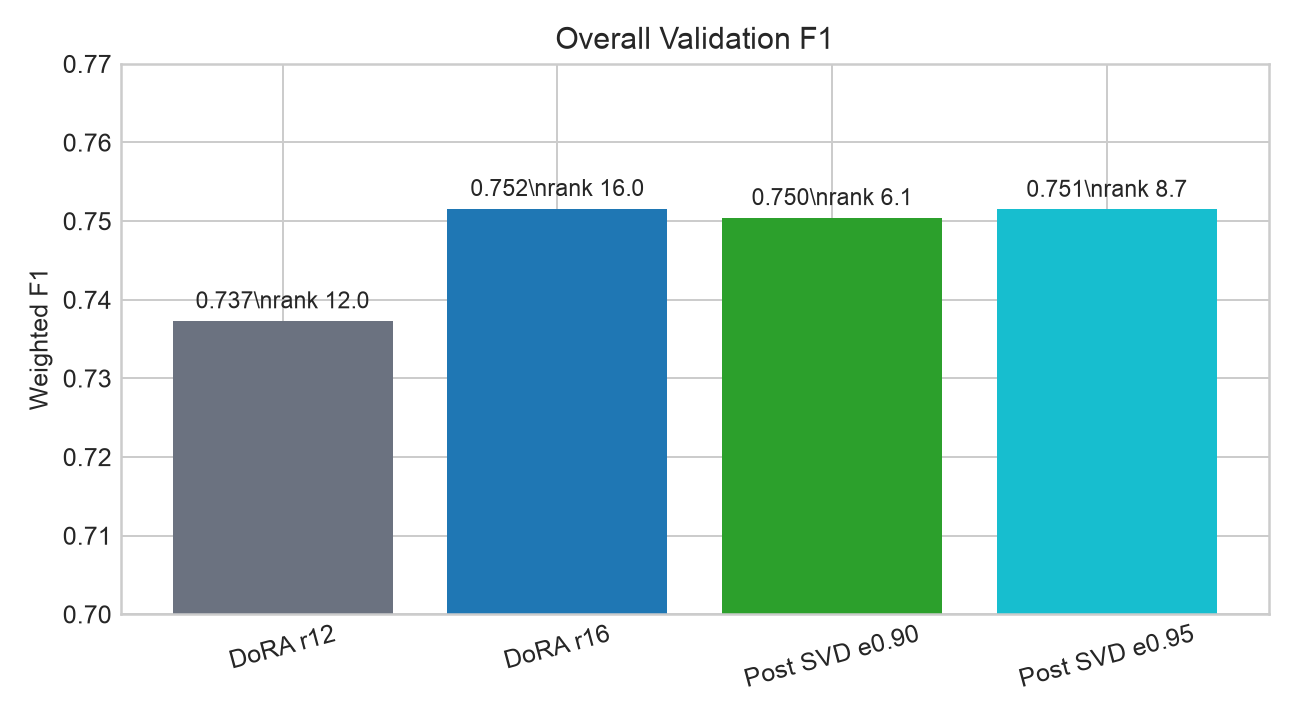
\includegraphics[width=0.68\linewidth]{figures/dora_svd_overall_f1.png}
\end{figure}

\[
\mathrm{DoRA}_{16}: F1=0.7516,\ r=16
\quad\Rightarrow\quad
\mathrm{SVD}_{0.95}: F1=0.7515,\ \bar r=8.68
\]
\end{frame}

\begin{frame}{Dataset-Level Result}
\begin{itemize}
  \item The result is consistent across SST-2 and IMDb.
  \item This suggests the compression is not only fitting one dataset.
\end{itemize}

\begin{figure}
    \centering
    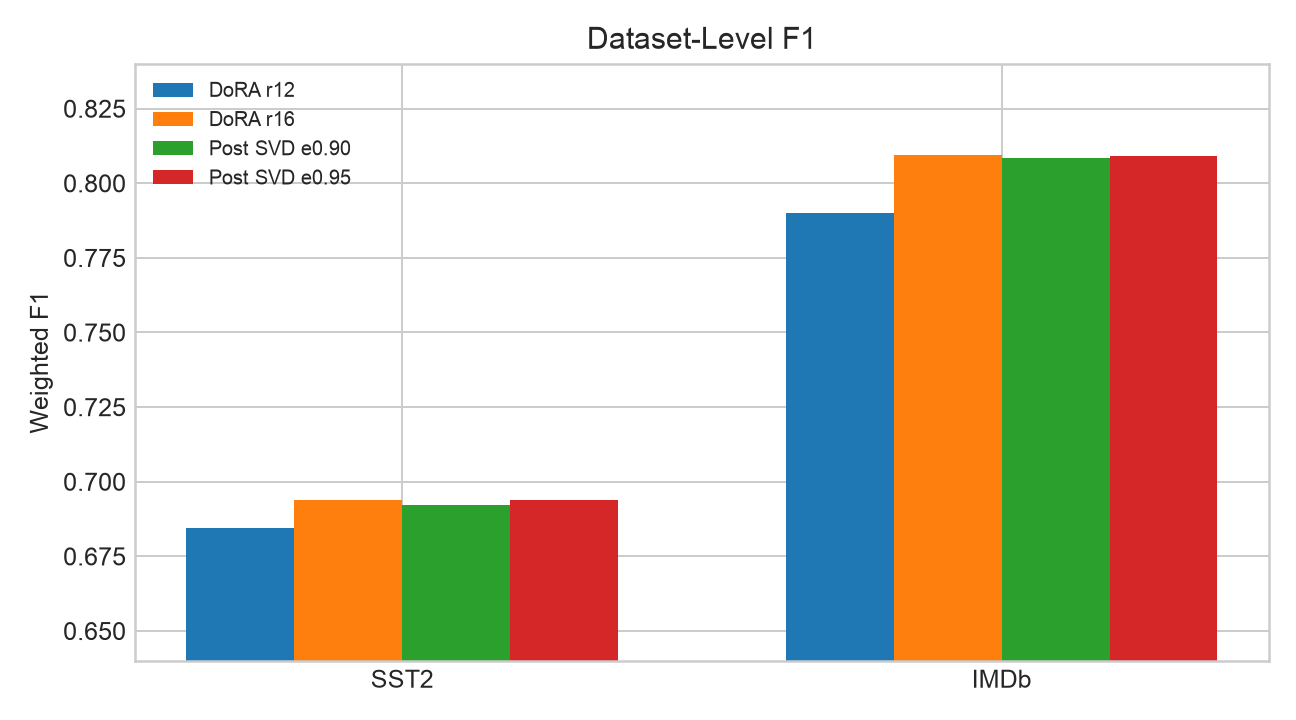
\includegraphics[width=0.68\linewidth]{figures/dora_svd_dataset_f1.png}
\end{figure}
\end{frame}

\begin{frame}{Compact Adapter Size Reduction}
\begin{itemize}
  \item Compact export stores only retained direction components.
  \item Energy 0.90 gives stronger compression; energy 0.95 is more conservative.
\end{itemize}

\begin{figure}
    \centering
    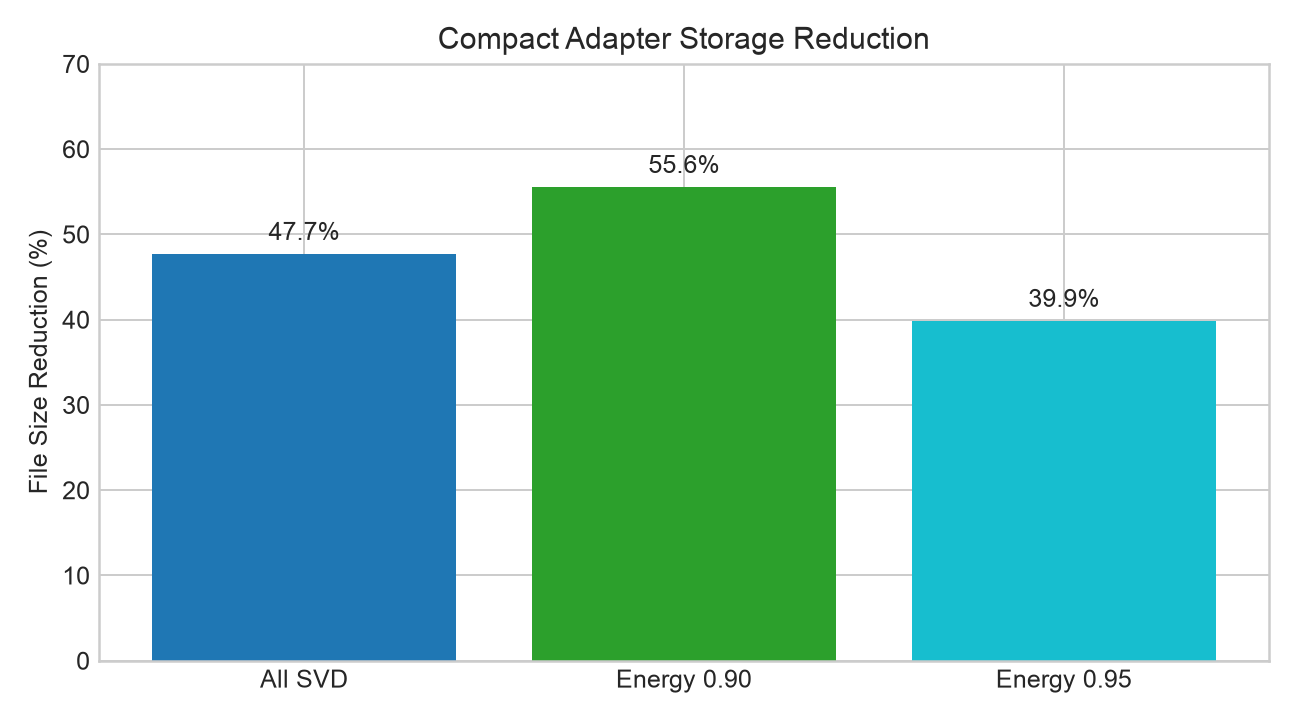
\includegraphics[width=0.58\linewidth]{figures/dora_svd_compact_reduction.png}
\end{figure}

\[
\tau=0.90:\ \mathrm{file}\downarrow55.6\%,
\qquad
\tau=0.95:\ \mathrm{file}\downarrow39.9\%
\]
\end{frame}

\begin{frame}{Compact Validation}
\begin{block}{Validation check}
The compact adapter is loaded and compared against the full-shape pruned adapter. A zero difference means the compact file represents the same adapter function.
\end{block}

\[
\widehat B_\ell\widehat A_\ell
\equiv
\operatorname{zeroPad}(\widehat B_\ell)
\operatorname{zeroPad}(\widehat A_\ell)
\]

\begin{table}
\centering
\small
\begin{tabular}{lr}
\toprule
Metric & Value \\
\midrule
Validated compact adapters & 72 / 72 \\
Max compact-vs-full F1 difference & 0.0 \\
Max tensor reconstruction difference & 0.0 \\
\bottomrule
\end{tabular}
\end{table}
\end{frame}

\begin{frame}{DoRA-SVD Takeaway}
\begin{block}{Main finding}
Post-training SVD reveals that trained DoRA direction updates contain redundant rank components.
\end{block}

\vspace{6pt}
\begin{itemize}
  \item Rank-16 DoRA can be compressed to average rank 8.68 with energy 0.95.
  \item Validation F1 remains nearly unchanged: \(0.7516 \rightarrow 0.7515\).
  \item Compact export reduces actual adapter file size by about 39.9\%.
  \item The magnitude branch remains untouched, so the method specifically targets the direction update.
\end{itemize}
\end{frame}


\end{document}
